\mysection{Il documento}

\myframe{Testo}{frame:testo}{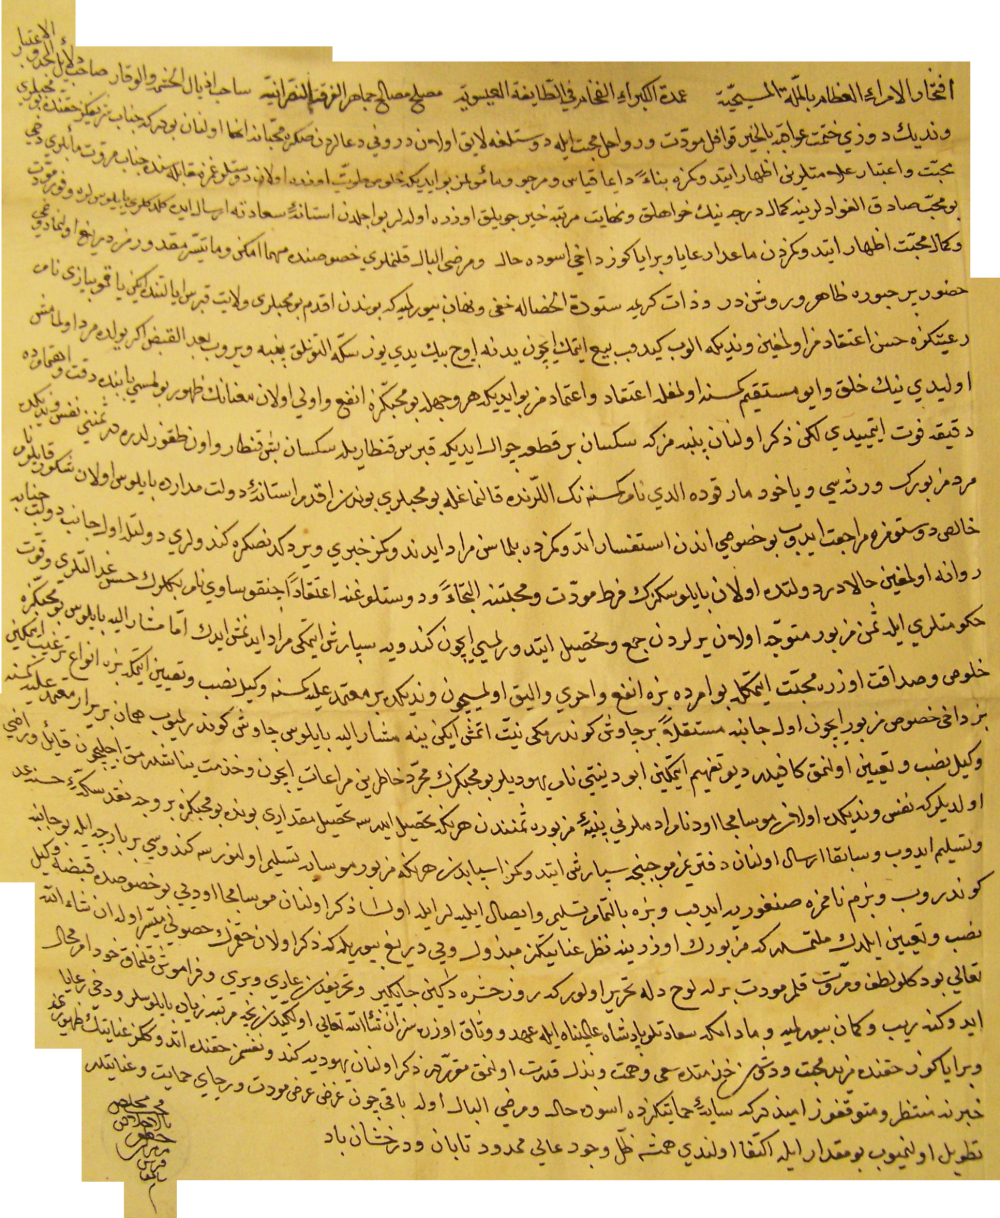
\includegraphics[scale=0.6]{testo.png}}

%% \myframe{Corrispondenti}{frame:corrispondenti}{
%%   \begin{tabular}{cc}
%%    \includegraphics[scale=0.3]{parole/cafertot-rid.jpg}&
%%    \includegraphics{parole/venedik_duzi.png}\\
%%    \spzrlvert[4.5cm]{mu.hibb  mu_halli.s bi-al-a_hlAqyy ^ga`afir  mIrimIrler qubris sAbiqAm} 
%%    & \footnotesize\spzrlvert[3cm]{:vened.Ik d.O^z:I} 
%%    \\
%% \end{tabular}}

\myframe{Cipro}{frame:kibris}{
\setarab
\novocalize
\begin{center}
\begin{tabular}{l@{\hspace{2cm}}r}
  \multicolumn{2}{c}{\includegraphics{parole/kibris_vilayet.png}}\\
  \spzrl{b.U mu.hiblarI wilAyat qubris ayAlatind:H .Jken}{}\\[1cm]
  \multicolumn{2}{c}{
    \parbox[c]{0.58\textwidth}{\centering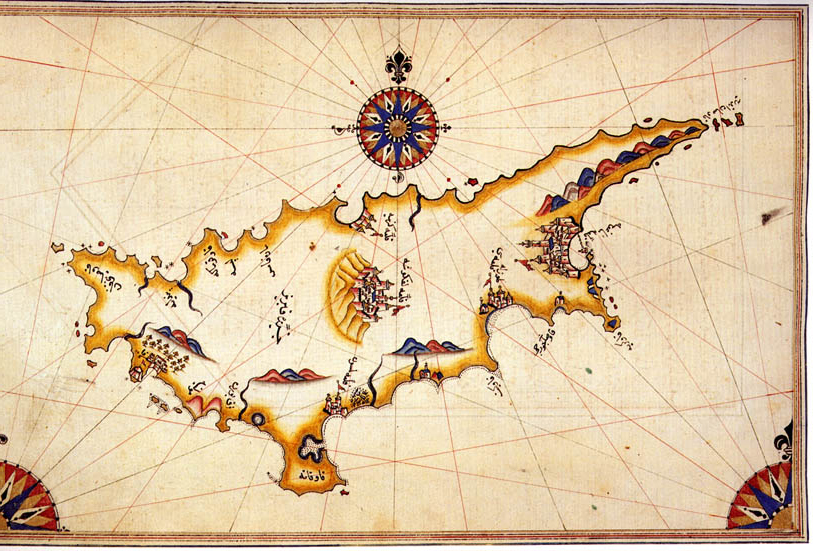
\includegraphics{atlas/Cyprus_by_Piri_Reis.jpg}}
    \parbox[c]{0.35\textwidth}{\tiny {\sc Piri Reis}, {\it Kitab-ı Bahriye}, 1521-25}}\\
\end{tabular}
\end{center}
}

%% \myframe{Giacomo Biasii}{frame:yaqumu}{
%% \setfarsi
%% \novocalize
%% \parbox[c]{0.48\textwidth}{
%%   \begin{tabular}{c}
%%     \includegraphics{parole/yaqum_biazii.png}\\
%%     \spzrl{y^Aqom.O||by^Az.Y nAm}\\
%%     \includegraphics{parole/rayetinize.png}\\
%%     \spzrl{ra`iyati^niz.H}\\
%% \end{tabular}}\hfill\parbox[c]{0.5\textwidth}{\centering
%%   \begin{tabular}{p{0.48\textwidth}}
%%     \includegraphics[scale=0.3]{documenti/vecellio321.png}
%%     \includegraphics[scale=0.3]{ritratti/mercante2.png}\\[0.2cm]
%%     {\tiny {\sc Cesare Vecellio}, {\it Habiti antichi et moderni di tutto il mondo}, Venezia, 1598}\\
%%   \end{tabular}}
%% }

%% \myframe{Cotone}{frame:penbe}{
%%   \setfarsi
%%   \novocalize
%%   \parbox[c]{0.4\textwidth}{\centering\begin{tabular}{c}
%%       \includegraphics{parole/penbe.png}\\[1cm]
%%       \spzrl{penb.H}\\[1cm]
%%   \end{tabular}}
%%   \hfill\parbox[c]{0.55\textwidth}{
%%     \begin{tabular}{c}
%%       \includegraphics[scale=0.6]{documenti/alpino.jpg}\\
%%       {\tiny {\sc Prosper Alpinus}, {\it De Plantis Aegypti Liber}, Venezia 1592}\\
%%   \end{tabular}}
%% }

\presspzrlvert[7cm]{Peso}{kantar}{kantar.png}
              {qubris  qan.tAr.Il.H seks^En  be^s qan.tAr wa .Qn .toq.Uz lodr.H}

%% \myframe{Peso}{frame:kantar}{
%%   \setfarsi
%%   \novocalize
%%   \begin{center}
%%     \begin{tabular}{c}
%%       \includegraphics{parole/kantar.png}\\[0.5cm]
%%       \spzrlvert[7cm]{qubris  qan.tAr.Il.H seks^En  be^s qan.tAr wa .Qn .toq.Uz lodr.H}\\
%%     \end{tabular}
%%   \end{center}
%% }


\myframe{Quantità}{frame:cuval}{
  \setfarsi
  \novocalize
  \parbox[c]{0.5\textwidth}{\centering\begin{tabular}{c}
      \includegraphics{parole/cuval.png}\\[1cm]
      \spzrlvert{seks^En  bir qi.ta`_H  ^cu:vAl}\\[1cm]
  \end{tabular}}
  \hfill\parbox[c]{0.4\textwidth}{
    \begin{tabular}{c}
      \includegraphics[scale=0.3]{documenti/luzerner.png}\\
      {\tiny {\sc Diebold Schillieg}, {\it Luzerner Chronik}, 1517}\\
  \end{tabular}}
}

\myframe{Prezzo}{sikke}{
  \begin{center}
  \begin{tabular}{c}
    \includegraphics{parole/sikke.png}\\[0.2cm]
    \spzrl{:W^c b.I^n yed.I y:Uz  sikk.H  alt.Unluq}\\[0.2cm]
    \includegraphics{monete/sanmatteo.png}\\[0.2cm]
    {\tiny Caravaggio, {\it Vocazione di San Matteo}, 1599-1600}\\
  \end{tabular}
  \end{center}
}

%% \myframe{A Venezia}{frame:venedige}{
%% \setarab
%% \novocalize
%% \begin{center}
%% \begin{tabular}{c}
%%   \includegraphics{parole/venedikte.png}\\[0.2cm]
%%   \spzrl{:vened.Ik.H  ^Al.Ub g.Id:Ub bay`i :Etm:a:k  .J^c:Un}\\[0.2cm]
%%   \includegraphics[scale=0.2]{atlas/venezia.png}\\
%%   {\tiny Bolognino Zaltieri, 1565}\\
%% \end{tabular}
%% \end{center}
%% }

%% %\presspzrlvert[7cm]{Peso}{kantar}{kantar.png}
%% %              {qubris  qan.tAr.Il.H seks^En  be^s qan.tAr wa .Qn .toq.Uz lodr.H}

%% \presspzrlvert{Eredi}{verese}{verese.png}
%%               {mord-i mazbUr:i_n wara_t:Hs.I}

%% \presspzrlvert{Marco d'Aldi}{marcodaldi}{marco_daldi.png}
%%               {m^Arq.O||d:H^Ald.I nAm}

